% #############################################################################
% This is Chapter 3
% !TEX root = ../main.tex
% #############################################################################
% Change the Name of the Chapter i the following line
\fancychapter{Problem Definition}
\cleardoublepage
\label{chap:problem}

This chapter defines the problem, the client requirements and lists the necessary services of a potential solution, which successfully addresses the problem.
First, some context surrounding the problem is given. Next, the profile of the target users is described. The following section lists the client requirements the solution must provide.
Then, it will shed the light on some essential concepts, to understand the services that need to be implemented. Lastly, it details some possible use case scenarios.

% -----------------------------------------------------
\section{Context}\label{chap:problem:context}

As discussed before, the same computers commonly used for communications and information storage are exploitable by attackers, and can cause minor inconveniences, to severe repercussions, such as, losing your confidential data to malicious parties.
This work focuses on an interesting approach to improve security, by adding another layer of security to communications, through the addition of a device, independent of the user's computer. The device is responsible for the security of sensitive data and communications.

% -----------------------------------------------------
\subsection{Entities}\label{chap:problem:entities}

These type of devices are especially relevant to people with high responsibility jobs, that handle very sensitive information, which have dire consequences if they are lost, corrupted or leaked.
Some examples are government officials who handle confidential information pertaining a country, company executives, such as the CEO with access to company secrets, diplomats who manage confidential treaties, and military officers who have access to information critical to national security.
Not just individuals could have an interest in these systems. A device can be assigned to a group of people representing an entity. For example, in the military, a device can be assigned to the navy, one to the infantry and so on. Any ranked officer, or person with a certain level of authority, could use the navy's device, to communicate with other entities, in behalf of the navy.

\subsection{Devices}\label{chap:problem:devices}

There are dedicated devices currently on the market, designed to secure communications and store private data.
These type of devices have physical tamper-resistant measures against attackers, who wish to read the device's information. They also provide fail-safe mechanisms in case of an attack.
HSM is a high grade device, with more computational power and larger storage capacity for secrets.
Smart Cards, provide secure and portable tamper-resistant storage. They have lower processing power, and a smaller memory. They have a lower cost, so can be produced in bulk and easily replaced.
Because of these features, they are widely used in the retail, healthcare, communication and government industries.

% -----------------------------------------------------
% -----------------------------------------------------
\section{Requirements}\label{chap:problem:requirements}

To effectively address the problem, there are several high-level requirements the solution must adhere to:
\begin{itemize}
	\item Devices should be distributable to individuals or entities, with more than one person;
	\item The system must allow communications between individuals, representing themselves or an entity;
	\item The system must be responsible for securing all communications against any attacks;
	\item The device should be independent from the user's personal computer;
	\item Users should be able to establish secure communications with new and existing entities;
	% \item New secure connections should be created, if existing communications are suspected to be compromised;
	\item It should provide an easy-to-use interface for non-technical people;
	\item It should have a relatively low cost, to allow distribution of several devices among multiple people;
	\item Only authorized individuals should be able to use the device.
\end{itemize}

These client requirements need to be translated into slightly more technical and tangible requirements. In order to secure communications, the solution should guarantee confidentiality, integrity and authentication.
Additionally with asymmetric keys, the system can provide non-repudiation to documents or files, by means of qualified digital signatures.
The device must securely store all keys, and perform all cryptographic operations pertaining the security of communications. Keys must never be exposed unencrypted to the outside.
Additionally, the device should have physical tamper-resistant measures and mechanisms in place, in case of an intrusion, such as, permanent erasure of all sensitive data. 
This means that even if an attacker is in possession of the physical device, it should be extremely difficult to extract any information from it.
The solution should work with a plethora of devices, in order to increase the adoptability of the solution among clients, or to be easily adapted in other projects.
The system should provide an application on the user's computer, which communicates with the physical device, and offers a simple interface to the its services, for the average non-technical user.
The system should use a common connection solution, e.g. USB cable, between the computer and device, to further increase adoptability.
In addition, the system should perform the services in a reasonable time, to minimize the wait, and improve the user experience.

% -----------------------------------------------------
% The solution should follow the PKCS \#11 standards, to strengthen its security requirements.
% This is where the widely established standard PKCS \#11 is again relevant. It allows operations to be standardized across different devices, increasing the range of supported devices.
% By implementing the system in accordance with these guidelines, it will have a higher device interoperability.

% -----------------------------------------------------
% -----------------------------------------------------
\section{Use Case Scenarios}\label{chap:problem:scenarios}

This section details use case examples the solution must cater to. Figure~\ref{fig:user:data-service} will be used as an example and illustration for the scenarios.

% -----------------------------------------------------
\subsection{User Authentication}\label{chap:problem:scenarios:auth}

Every user must authenticate himself before using the device. This can be done by providing a PIN, which the device will verify, before unlocking the user's session.
The device will come from fabric with a default authentication PIN. The users should be allowed to change this number.
For personal devices there is only one user, the owner, as illustrated by Bob in figure~\ref{fig:user:data-service}. There is only a single authentication PIN, which when sent to the device, unlocks the session, and the user can access its services.
For groups and entities there can be multiple users, illustrated by Alice. In this case, there are different scenarios for authentication.
The simplest is when the individual user does not need to authenticate himself, only the entity. There is only a single authentication PIN for the entity. All the user's with permission to communicate in behalf of the entity, must know the PIN.
The second scenario, is when an entity wishes to authenticate each individual user, with access to the device. 
This entails a more complex process. A specific user is assigned the role of administrator. For example in the military, this could be assigned to the top ranking general. The administrator, using the administrator PIN, is able to register new users with their own private PIN, access the logs of which user logged in and when, as well as, which messages they sent and received.
The registration of a new user can be done physically with both administrator and user present. Afterwards, the registered user can use their credentials to authenticate himself, and use the device to communicate, in behalf of the entity.
It is important to note that in all scenarios, only the users or the entity is authenticated, the device does not authenticate itself to the user.
% The administrator authenticates himself to the device, begins the registration process and allows the user to insert their name and PIN.

% -----------------------------------------------------
\subsection{Secure Communications}\label{chap:problem:scenarios:comms}

%% SECURE COMMUNICATIONS %%
The main goal of the system is to enable secure communications. Communications can be setup between two or more entities. For each configured communication, the same symmetric key is securely stored in each device. One key per communication.
For a user to send secure data, first he authenticates himself to the device, then sends the data to it. The device will return it secured. The user can then send it through a convenient offline service such as email, or an online chat service. Only a recipient with a similar device and the same key can read the original contents.

\begin{figure}[h!]
    \centering
    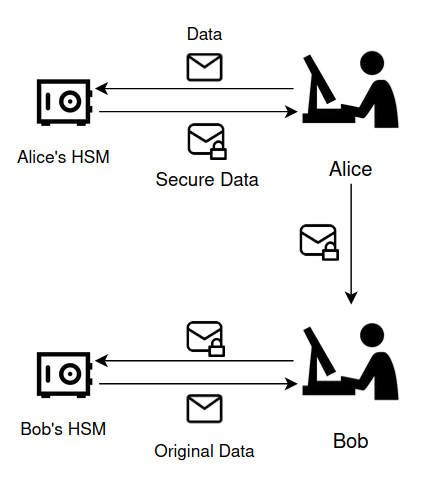
\includegraphics[width=0.7\textwidth]{./Images/user-data-service.png}
    \caption{Secure data exchange service example using internal keys}
    \label{fig:user:data-service}
\end{figure}

%% USAGE EXAMPLE %%
A possible usage example of secure data exchange between two users, Alice and Bob, is depicted in figure \ref{fig:user:data-service}. Firstly, Alice forwards the data, to be sent securely to Bob, to the device and the device returns the data secured with an internal key. Then, Alice can forward the result to any entity with the same internal key in their device, through a chat application, e-mail or other convenient service.
Upon receiving the secure message from Alice, Bob sends it to the device, and receives the original message back.
This service must prevent any third party from gaining access to the data, or altering the message. The receiver can be confident of the data's origin. It could not have been sent by any malicious entity.

%% INITIAL STATE, FABRIC CONFIGURATION %%
Each entity, upon ordering the device, should be able to specify which entities it wants to communicate with.
For example, Alice can request a device which enables two separate communication channels with Bob and Charlie, separately. Alice can also request a single channel with all three entities. In this case, only one shared key is required for all.
Before devices are delivered, the keys will be generated and stored in the necessary device. When all involved entities receive their device, they can begin secure communications immediately.
%% COMMUNICATION CHANNELS LIMIT %%
The device should not have a practical limit on the amount communication channels it can establish. This means it should have a reasonable amount of key storage space, for communications with enough different entities.
If the device's secure storage is limited, then a solution using symmetric or asymmetric keys to secure all other keys on a higher capacity non-volatile memory.
This gives entities the flexibility needed to communicate with the number of entities they choose.

%% QUALIFIED DIGITAL SIGNATURES %%
Another possible use case scenario is the inclusion of a pair of asymmetric keys, generated inside each device, and never exposed to the outside. This allows the generation of qualified digital signatures, which can legally represent the entity.
Then, when a user wishes to generate a signature for a piece of data, he must send the data to the device, which computes and returns the qualified signature.
% Each device has a pair of asymmetric keys stored in secure storage, generated inside the device from fabric. These keys allow the storage of a practically unlimited number of symmetric keys in non-volatile memory.
% This feature is useful in other situations. There are cases where existing symmetric keys might need to be revoked, due to suspicion of being compromised, with new ones generated and shared.
% Another case is if the symmetric key has an expiration date, when it expires, new keys need to be exchanged.

% Finally, when using asymmetric keys, beyond providing authentication to the communications, the data sender can be authenticated to the receiver, using the entities private key stored in the device.

% -----------------------------------------------------
\subsection{New Communications}\label{chap:problem:scenarios:keys}

%% REASONING FOR SERVICE %%
The operations described so far provide a usable and functional system to organizations and users, but it is not very flexible. It does not allow users to communicate with new entities, without returning the device to manufacturing, to be equipped with the necessary information.
To avoid this, a service should be available to users with production devices in their possession, to securely trade data with another entity with an identical device, which the device previously could not. It should be easy to provide the functionality without burdening the user with additional responsibility.
%% SERVICE PRESENTATION %%
A possible solution is the inclusion of a control station, where entities originally collect their devices. Each device is delivered with its own communication channel with the control station. This station is effectively treated as a special entity.
Whenever users wish to communicate with another user, they can send a list of entities they intend to communicate with to the station, secured with the data exchange service. The control station subsequently supplies the user with the necessary information, to be imported in their device.

\begin{figure}[h]
    \centering
    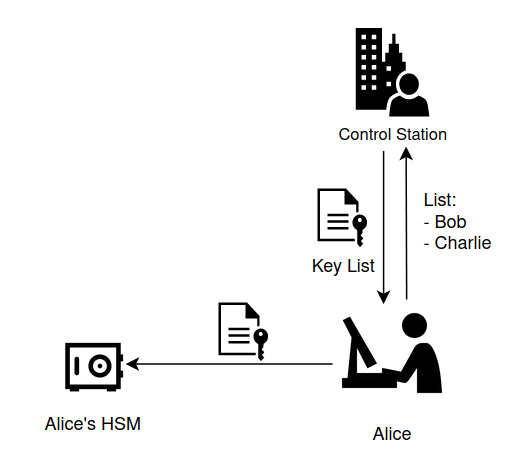
\includegraphics[width=0.65\textwidth]{./Images/user-import-service.png}
    \caption{Import key list to device usage example}
    \label{fig:user:import-service}
\end{figure}

%% USAGE EXAMPLE %%
A use case scenario of this service is depicted in figure \ref{fig:user:import-service}.
Alice forwards the list with the names of entities to the control station, which returns the key list to Alice. The list can be forwarded to the device, where the new keys are stored.
Alice can then start communications with Bob and Charlie, using the secure data exchange service, as soon as everyone imports the list into their respective devices.
%% ADVANTAGES / POSSIBILITIES %%
The service offers the possibility of setting up a regular communication update schedule. It grants the flexibility of key revocation when needed, data exchange with new entities, as well as updating communication keys, which have reached their expiration date, with no additional complexity to the user.
A regular update schedule, adds longevity to the system. It avoids overuse, and reduces the possibility of compromised connections. When keys reach the expiration date, new ones can be distributed.
A less cumbersome possibility for the user, is whenever an entity is added to system and receives their device, the station delivers a message to each entity, with the updated key list. The list can be imported by each user if needed.

% The list can be sent using an offline service such as email. Every time a new entity is added to the list, the station sends a new email with the updated list. Each entity can get access these updates when they need it.

% Each month an entity can hand over a list of the entities it wishes to communicate with to the control station, which will accordingly yield the corresponding key set, as pictured in figure \ref{fig:user:import-service}.
% Each entity only needs to forwards the list to the device, and the new keys are immediately stored and ready to be used.


% The list can be provided at the manufacturing control station, when the device is delivered.
% Afterwards, there are two options to distribute the list. When the list is updated with new entities, a member of the entity will physically go to the station, to retrieve it.
% Alternatively, the entity will receive the device with the necessary keys to securely communicate with the control station. When an entity needs the list, it will be supplied for them by the control station. In this scenario, the control station can be thought of as a special entity.

% Adding to the previous scenario with asymmetric keys, users will be able to establish secure communications with new entities. This is achieved by distributing a list of available entities to communicate with.
% When and individual, e.g. Alice, wants to establish communications with a new entity, such as Bob, she needs to get Bob's key from the received list. Then they can securely trade a new key, and begin communications.

% -----------------------------------------------------
% -----------------------------------------------------
\section*{Summary}\label{chap:problem:summary}

This chapter defines the context for the addition of a device, independent of a personal computer, which secures communications between entities, such as the military or government.
The fundamental and non-technical requirements for an adequate solution were defined, such as, its characteristics, capabilities and usability. In short, the system should be composed of a user-friendly and low cost device, easily distributed among individuals or groups, and provide secure communications between them.
Several possible use case scenarios for the system were identified.
The system could be used to authenticate a user to the device, to allow access to its secure communication capabilities. The system must allow communications between entities with identical devices, by the means of a personal computer connected to the device, which secures the messages before transmission.
The system could also allow the establishment of communications with new entities, by employing a control station which, when necessary, distributes the essential information among all entities, to allow new secure communication channels.
